$K$D-tree is a space partitioning structure that can be used to organise data points in $k$ dimensional space. In this project, we limit the dimension $k$ to be $2$. We implement the $K$D-tree as a binary tree in which every node is a $2$-dimensional point. Every non-leaf node is representing a splitting line that divides the space into two parts. Then every points to the left (or down) of this line are represented by the left subtree and points to the right (or up) of this line are represented by the right subtree. In Fig. \ref{fig:kd_tree_example} we illustrate an example of $K$D-tree.

\begin{figure}
     \centering
     \begin{subfigure}[b]{0.58\textwidth}
         \centering
         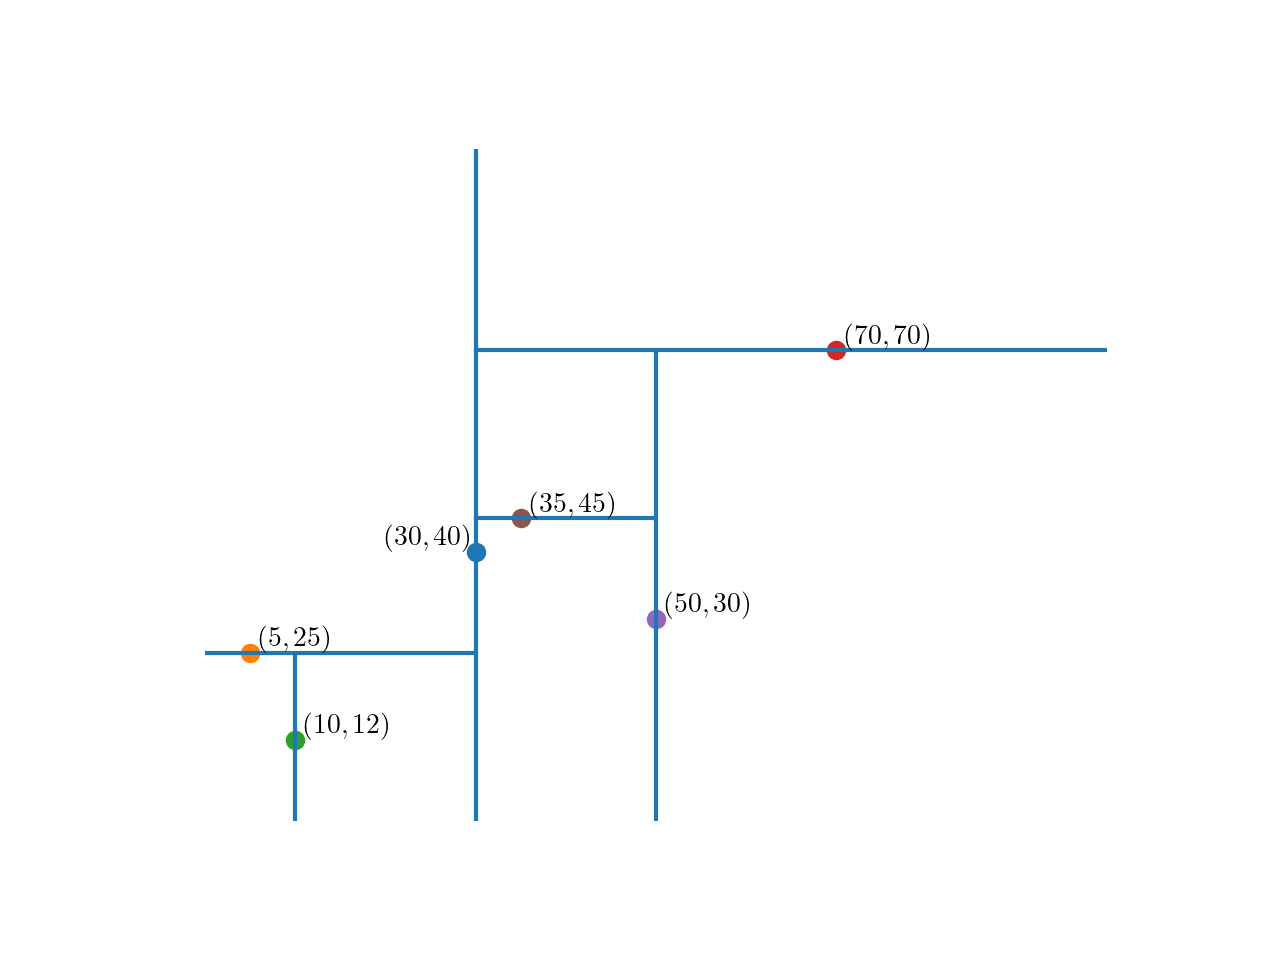
\includegraphics[width=\textwidth]{graphs/implementation/2d/kdtree_partition}
         \caption{The $2$D space and the partition of $K$D-tree}
         \label{fig:y equals x}
     \end{subfigure}
     \hfill
     \begin{subfigure}[b]{0.40\textwidth}
         \centering
         \begin{tikzpicture}
\tikzstyle{bplus}=[rectangle split, rectangle split horizontal,rectangle split ignore empty parts,draw]
\tikzstyle{every node}=[bplus]
\tikzstyle{level 1}=[sibling distance=30mm]
\tikzstyle{level 2}=[sibling distance=15mm]
\node {(30,40)} [->]
  child {node {(5,25)}
    child {node {(10,12)}}
    child[missing]{}    
  } 
  child {node {(70,70)}
    child {node {(50,30)}
    	child {node {(35,45)}}
    	child[missing]{}
    }
    child[missing]{}
  }
;\end{tikzpicture}
         \caption{The tree structure of the $K$D-tree}
         \label{fig:three sin x}
     \end{subfigure}
        \caption{An example of $K$D-Tree}
        \label{fig:kd_tree_example}
\end{figure}

\subsubsection{Insertion of $K$D-tree}

Similar to a binary search tree, we need to traverse the tree when we need to insert a point to the $K$D-tree. The only difference is that we need to switch the axes when inserting into a $K$D-tree. For example, since the dimension is $2$ in our case, we compare the $x$-coordinate at the root level. Then in the root's direct children, we compare the $y$-coordinate at that level. Formally, the insertion algorithm is expressed as in Algo. \ref{algo:kd-tree-insertion}.

\begin{algorithm}[H]
\SetAlgoLined
\SetKwInOut{Input}{input}
\Input{\texttt{t}: The node to be inserted; \texttt{k}: The key to be inserted; \texttt{cd}: Current dimension}
\KwResult{\texttt{t}: The node with the inserted key \texttt{k}}
	\texttt{DIM=2;}\\
	\uIf{\texttt{t==NULL}} {
		\texttt{t = NewNode(k)}
	}
	\uElseIf{\texttt{x[cd]<t.data[cd]}} {
		\texttt{t.left=insert(x, t.left, (cd+1) \% DIM )}
	}
	\uElse{
		\texttt{t.right=insert(x, t.right, (cd+1)\% DIM)}
	}
 	\Return \texttt{N}
 \caption{$K$D-tree Insertion}
 \label{algo:kd-tree-insertion}
\end{algorithm}

To insert a key \texttt{k} into the $K$D-tree with \texttt{T} as its node, we only need to apply this function with the root node as \texttt{insert(T, k, 0)}. 

In the Algo. \ref{algo:kd-tree-insertion}, the insertion of a key is performed in the following steps:

\begin{enumerate}
	\item On Line $1$, we specify the dimension to be $2$.
	\item Then we first check if the node is \texttt{NULL}. If it is \texttt{NULL}, which means we should have a new leaf node, then we create a new node and give it our key.
	\item Otherwise, from Line $4$ to $7$, we check the data at current dimension. If it is smaller than the data in the node \texttt{t} at current dimension, then we should insert into the left subtree. Otherwise, we should insert into the right subtree.
	\item When we moves down to the left or right subtree, we switch the current dimension by calculating \texttt{(cd+1)\% DIM}.
\end{enumerate}

\begin{mscexample}
	In Fig. \ref{fig:kd_tree_example}, we present an example of $K$D-tree. In this example, we will illustrate how it is constructed. Assume our data points is $$[(30,40), (5,25), (10,12), (70,70), (50,30), (35,45)]$$
	
	The construction of the $K$D-tree follows the steps below:
	
	\begin{enumerate}
		\item We start with $(30,40)$ by creating a new node and give it the data point, which results in the root node in the figure.
		\item After that we insert $(5,25)$, since \texttt{x[0]<t.data[0]}, we insert this node as the left subtree to the root.
		\item Then we insert $(10, 12)$. First we compare the $x$-coordinate at the root level. As $10<30$, we go to the left subtree. Then we compare at the root's children level and compare the $y$-coordinate. As $12<25$, we go to the left subtree and create a new node there.
		\item Similarly, we insert other keys one-by-one.
	\end{enumerate}
	
\end{mscexample}